\chapter{最短経路}

\index{最短経路}

グラフの2ノード間の最短経路を求めることは重要なトピックであり様々な応用が可能です。
例えば,複数の都市があり、それぞれをつなぐ道路の長さが与えられたときに,
ある2つの都市を結ぶ路線の最短距離を計算する、などです。
重みのないグラフでは、パスの長さはその辺の数に等しいので、単純な幅優先探索(BFS)で最短経路を求めることができます。

この章では、重み付きグラフで最短経路を見つけるための洗練されたアルゴリズムをみていきます。

\section{最短経路(Bellman–Ford)}

\index{最短経路(Bellman–Ford)}

\key{Bellman–Ford algorithm}\footnote{The algorithm is named after
R. E. Bellman and L. R. Ford who published it independently
in 1958 and 1956, respectively \cite{bel58,for56a}.} はあるノードから開始して
全てのノードへの最短経路を計算します。
このアルゴリズムは負のコストとなる閉路を持たない全てのグラフで利用できます。
もし、負のコストとなる閉路が存在する場合、その検出を行います。

このアルゴリズムは、開始ノードからすべてのノードまでの距離を調べます。
まず、開始ノードまでの距離は0であり、他のすべてのノードまでの距離は無限とします。
そして、どの距離も小さい距離に更新できなくなるまで、より小さな距離に更新できる辺を見つけていきます。

\subsubsection{Example}

次の図でBellman–Fordアルゴリズムの動作を説明します。
\begin{center}
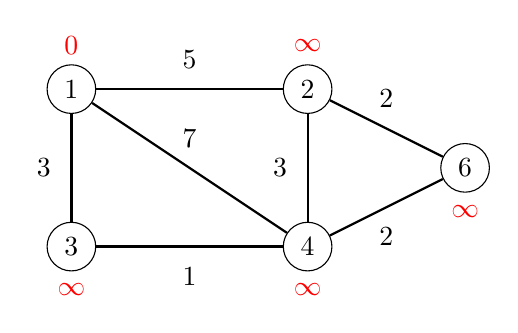
\begin{tikzpicture}
\node[draw, circle] (1) at (1,3) {1};
\node[draw, circle] (2) at (4,3) {2};
\node[draw, circle] (3) at (1,1) {3};
\node[draw, circle] (4) at (4,1) {4};
\node[draw, circle] (5) at (6,2) {6};
\node[color=red] at (1,3+0.55) {$0$};
\node[color=red] at (4,3+0.55) {$\infty$};
\node[color=red] at (1,1-0.55) {$\infty$};
\node[color=red] at (4,1-0.55) {$\infty$};
\node[color=red] at (6,2-0.55) {$\infty$};
\path[draw,thick,-] (1) -- node[font=\small,label=above:5] {} (2);
\path[draw,thick,-] (1) -- node[font=\small,label=left:3] {} (3);
\path[draw,thick,-] (3) -- node[font=\small,label=below:1] {} (4);
\path[draw,thick,-] (2) -- node[font=\small,label=left:3] {} (4);
\path[draw,thick,-] (2) -- node[font=\small,label=above:2] {} (5);
\path[draw,thick,-] (4) -- node[font=\small,label=below:2] {} (5);
\path[draw,thick,-] (1) -- node[font=\small,label=above:7] {} (4);
\end{tikzpicture}
\end{center}
各ノードは距離を持ちます。
開始ノードの距離は0と、それ以外の距離はINFです。

このアルゴリズムでは、あるノードから隣接するノードの距離を縮めることのできる辺を調べます。
まず、ノード1から始めます。全ての隣接ノードへの距離は(初期値がINFなので)縮まります。
\begin{center}
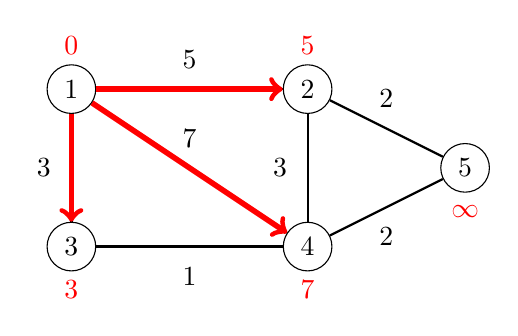
\begin{tikzpicture}
\node[draw, circle] (1) at (1,3) {1};
\node[draw, circle] (2) at (4,3) {2};
\node[draw, circle] (3) at (1,1) {3};
\node[draw, circle] (4) at (4,1) {4};
\node[draw, circle] (5) at (6,2) {5};
\node[color=red] at (1,3+0.55) {$0$};
\node[color=red] at (4,3+0.55) {$5$};
\node[color=red] at (1,1-0.55) {$3$};
\node[color=red] at (4,1-0.55) {$7$};
\node[color=red] at (6,2-0.55) {$\infty$};
\path[draw,thick,-] (1) -- node[font=\small,label=above:5] {} (2);
\path[draw,thick,-] (1) -- node[font=\small,label=left:3] {} (3);
\path[draw,thick,-] (3) -- node[font=\small,label=below:1] {} (4);
\path[draw,thick,-] (2) -- node[font=\small,label=left:3] {} (4);
\path[draw,thick,-] (2) -- node[font=\small,label=above:2] {} (5);
\path[draw,thick,-] (4) -- node[font=\small,label=below:2] {} (5);
\path[draw,thick,-] (1) -- node[font=\small,label=above:7] {} (4);

\path[draw=red,thick,->,line width=2pt] (1) -- (2);
\path[draw=red,thick,->,line width=2pt] (1) -- (3);
\path[draw=red,thick,->,line width=2pt] (1) -- (4);
\end{tikzpicture}
\end{center}

次に
$2 \rightarrow 5$ と $3 \rightarrow 4$
の2つの辺が距離を縮めます。
\begin{center}
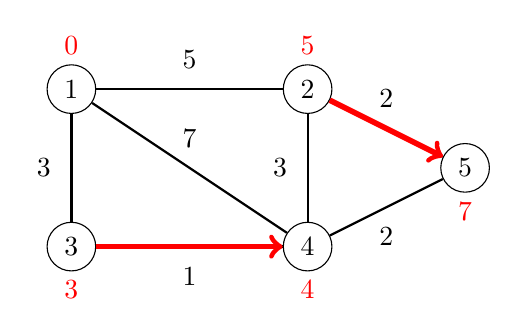
\begin{tikzpicture}
\node[draw, circle] (1) at (1,3) {1};
\node[draw, circle] (2) at (4,3) {2};
\node[draw, circle] (3) at (1,1) {3};
\node[draw, circle] (4) at (4,1) {4};
\node[draw, circle] (5) at (6,2) {5};
\node[color=red] at (1,3+0.55) {$0$};
\node[color=red] at (4,3+0.55) {$5$};
\node[color=red] at (1,1-0.55) {$3$};
\node[color=red] at (4,1-0.55) {$4$};
\node[color=red] at (6,2-0.55) {$7$};
\path[draw,thick,-] (1) -- node[font=\small,label=above:5] {} (2);
\path[draw,thick,-] (1) -- node[font=\small,label=left:3] {} (3);
\path[draw,thick,-] (3) -- node[font=\small,label=below:1] {} (4);
\path[draw,thick,-] (2) -- node[font=\small,label=left:3] {} (4);
\path[draw,thick,-] (2) -- node[font=\small,label=above:2] {} (5);
\path[draw,thick,-] (4) -- node[font=\small,label=below:2] {} (5);
\path[draw,thick,-] (1) -- node[font=\small,label=above:7] {} (4);

\path[draw=red,thick,->,line width=2pt] (2) -- (5);
\path[draw=red,thick,->,line width=2pt] (3) -- (4);
\end{tikzpicture}
\end{center}

最後にもう1つ更新できます。
\begin{center}
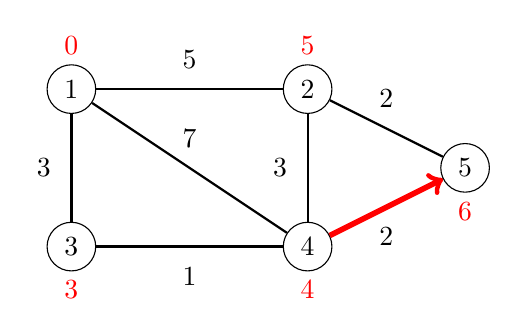
\begin{tikzpicture}
\node[draw, circle] (1) at (1,3) {1};
\node[draw, circle] (2) at (4,3) {2};
\node[draw, circle] (3) at (1,1) {3};
\node[draw, circle] (4) at (4,1) {4};
\node[draw, circle] (5) at (6,2) {5};
\node[color=red] at (1,3+0.55) {$0$};
\node[color=red] at (4,3+0.55) {$5$};
\node[color=red] at (1,1-0.55) {$3$};
\node[color=red] at (4,1-0.55) {$4$};
\node[color=red] at (6,2-0.55) {$6$};
\path[draw,thick,-] (1) -- node[font=\small,label=above:5] {} (2);
\path[draw,thick,-] (1) -- node[font=\small,label=left:3] {} (3);
\path[draw,thick,-] (3) -- node[font=\small,label=below:1] {} (4);
\path[draw,thick,-] (2) -- node[font=\small,label=left:3] {} (4);
\path[draw,thick,-] (2) -- node[font=\small,label=above:2] {} (5);
\path[draw,thick,-] (4) -- node[font=\small,label=below:2] {} (5);
\path[draw,thick,-] (1) -- node[font=\small,label=above:7] {} (4);

\path[draw=red,thick,->,line width=2pt] (4) -- (5);
\end{tikzpicture}
\end{center}


これ以上は距離を縮めることはできません。
つまり、開始ノードからの最短距離が確定したことを意味します。

例えば、ノード1からノード5までの最短距離3は、次のような経路となりました。

\begin{center}
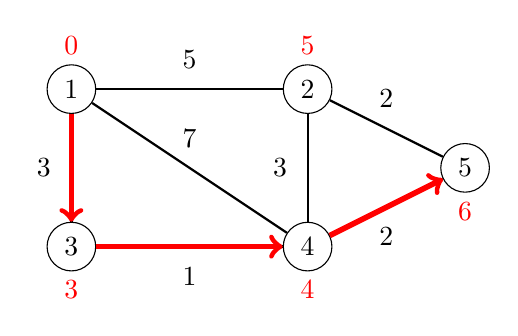
\begin{tikzpicture}
\node[draw, circle] (1) at (1,3) {1};
\node[draw, circle] (2) at (4,3) {2};
\node[draw, circle] (3) at (1,1) {3};
\node[draw, circle] (4) at (4,1) {4};
\node[draw, circle] (5) at (6,2) {5};
\node[color=red] at (1,3+0.55) {$0$};
\node[color=red] at (4,3+0.55) {$5$};
\node[color=red] at (1,1-0.55) {$3$};
\node[color=red] at (4,1-0.55) {$4$};
\node[color=red] at (6,2-0.55) {$6$};
\path[draw,thick,-] (1) -- node[font=\small,label=above:5] {} (2);
\path[draw,thick,-] (1) -- node[font=\small,label=left:3] {} (3);
\path[draw,thick,-] (3) -- node[font=\small,label=below:1] {} (4);
\path[draw,thick,-] (2) -- node[font=\small,label=left:3] {} (4);
\path[draw,thick,-] (2) -- node[font=\small,label=above:2] {} (5);
\path[draw,thick,-] (4) -- node[font=\small,label=below:2] {} (5);
\path[draw,thick,-] (1) -- node[font=\small,label=above:7] {} (4);

\path[draw=red,thick,->,line width=2pt] (1) -- (3);
\path[draw=red,thick,->,line width=2pt] (3) -- (4);
\path[draw=red,thick,->,line width=2pt] (4) -- (5);
\end{tikzpicture}
\end{center}

\subsubsection{実装}

ノード$x$からグラフの全ノードまでの最短距離を求める実装を以下に示します。
この実装は、グラフが $(a, b, w)$ というタプルのリスト \texttt{edges} で表現されているとします。
それぞれの要素は辺を表し、ノード $a$ からノード $b$向きに重み $w$ の辺とします。
Bellman–Fordは$n - 1$ラウンドで構成されます。各ラウンドはグラフのすべてのエッジを調べ、隣接ノードへの距離を縮めようと試みます。
実装では,始点$x$ からグラフの全ノードまでの距離を格納する配列 \texttt{distance} を定義します。なお、定数 \texttt{INF} は,無限遠を表します.

\begin{lstlisting}
for (int i = 1; i <= n; i++) distance[i] = INF;
distance[x] = 0;
for (int i = 1; i <= n-1; i++) {
    for (auto e : edges) {
        int a, b, w;
        tie(a, b, w) = e;
        distance[b] = min(distance[b], distance[a]+w);
    }
}
\end{lstlisting}

時間計算量を考えると、先に述べた通り、$n - 1$ 回のラウンドで構成され,各ラウンドで $m$ 個の辺をすべて繰り返し処理するので,
$O(nm)$となります。
グラフに負の閉路が存在しない場合、
最も長い最短パスが$n - 1$の辺で構成されていても、$n - 1$回のラウンドで確定します。
多くの場合、$n - 1$ラウンドよりも早く求められるのが普通でしょう。
そのため、あるラウンドで距離を縮めることができなければ、アルゴリズムを打ち切るとより効率的なアルゴリズムになるでしょう。

\subsubsection{負の閉路 - Negative cycles}

\index{negative cycle}

また、Bellman - Ford アルゴリズムは、グラフに負の閉路が含まれているかどうかを確認するために使用することができます。
以下に例を示します。
\begin{center}
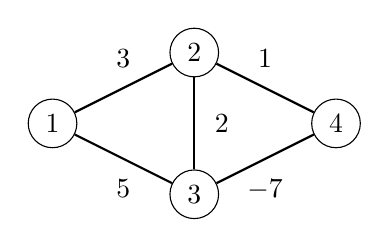
\begin{tikzpicture}[scale=0.9]
\node[draw, circle] (1) at (0,0) {$1$};
\node[draw, circle] (2) at (2,1) {$2$};
\node[draw, circle] (3) at (2,-1) {$3$};
\node[draw, circle] (4) at (4,0) {$4$};

\path[draw,thick,-] (1) -- node[font=\small,label=above:$3$] {} (2);
\path[draw,thick,-] (2) -- node[font=\small,label=above:$1$] {} (4);
\path[draw,thick,-] (1) -- node[font=\small,label=below:$5$] {} (3);
\path[draw,thick,-] (3) -- node[font=\small,label=below:$-7$] {} (4);
\path[draw,thick,-] (2) -- node[font=\small,label=right:$2$] {} (3);
\end{tikzpicture}
\end{center}
\noindent
グラフに長さ$-4$の負の閉路
$2 \rightarrow 3 \rightarrow 4 \rightarrow 2$
があるとしましょう。

グラフに負がある場合、無限回にそのサイクルに関係するノードの距離は小さくなっていきます。
つまり、最短経路という概念は意味をなさないともいえます。
負の閉路は、$Bellman–Ford$ を使用して、アルゴリズムを$n$ラウンド実行することによって検出することができます(訳註: $n-1$ではないことに注意)。
この追加ラウンドで距離が縮まれば、そのグラフは負の閉路を含むことになります。
そしてこれは、開始ノードに関係なく、グラフ上の負の閉路を探索することができます。

\subsubsection{SPFAアルゴリズム - SPFA algorithm}

\index{SPFA algorithm}

\key{SPFA アルゴリズム} (''Shortest Path Faster Algorithm'') \cite{fan94}は、
Bellman-Fordアルゴリズムの亜種ですが、多くの場合より効率的です。
SPFAアルゴリズムは、各ラウンドですべての辺を通過するのではなく、より賢く見るべき辺を選択します。

このアルゴリズムでは、距離を更新しうる可能性のあるノードをキューとして持ちます。
まず、アルゴリズムは開始ノードxをキューに追加します。
処理では常にキューの最初のノードをみて、$a \rightarrow b$が距離を更新すると、ノード$b$をキューに追加します。
SPFAアルゴリズムの効率はグラフの構造に依存します。


% 訳註: このコードはなぜかコメントアウトされていた
%
% The following implementation uses a
% \texttt{queue} \texttt{q}.
% In addition, an array \texttt{inqueue} indicates
% if a node is already in the queue,
% in which case the algorithm does not add
% the node to the queue again.
%
% \begin{lstlisting}
% for (int i = 1; i <= n; i++) distance[i] = INF;
% distance[x] = 0;
% q.push(x);
% while (!q.empty()) {
%     int a = q.front(); q.pop();
%     inqueue[a] = false;
%     for (auto b : v[a]) {
%         if (distance[a]+b.second < distance[b.first]) {
%             distance[b.first] = distance[a]+b.second;
%             if (!inqueue[b]) {q.push(b); inqueue[b] = true;}
%         }
%     }
% }
% \end{lstlisting}

このアルゴリズムは多くの場合効率的ですが、最悪の場合の時間計算量は依然として$O(nm)$で、
Bellman-Fordと同変わらない処理時間となる入力が作成可能です。

\section{ダイクストラ法 - Dijkstra's algorithm}

\index{Dijkstra's algorithm}

\key{Dijkstra's法} \footnote{E. W. Dijkstra published the algorithm in 1959 \cite{dij59}}
は、ベルマン-フォードと同様に、始点ノードからグラフの全ノードまでの最短経路を求める手法です。
ダイクストラ法は、より大規模なグラフの処理に使用できます。
注意すべき点として、このアルゴリズムはグラフ内に負の重みのエッジが存在しないことが必須の条件です。

ベルマンフォードと同様に、ダイクストラ法は各ノードまでの距離を維持して、探索中に距離を更新していきます。
ダイクストラ法では、グラフに負のエッジがないことを利用して、各エッジをただ一度だけ処理するので高速に動作します。

\subsubsection{例}
次のグラフで、ノード1を始点とするとき、Dijkstraのアルゴリズムがどのように働くかをみていきます。

\begin{center}
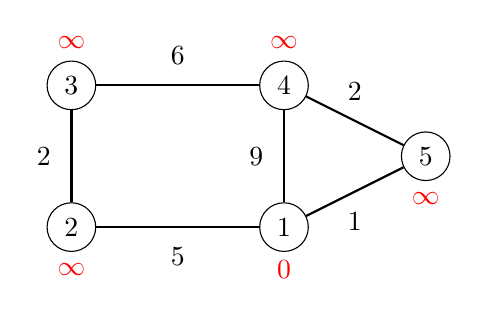
\begin{tikzpicture}[scale=0.9]
\node[draw, circle] (1) at (1,3) {3};
\node[draw, circle] (2) at (4,3) {4};
\node[draw, circle] (3) at (1,1) {2};
\node[draw, circle] (4) at (4,1) {1};
\node[draw, circle] (5) at (6,2) {5};

\node[color=red] at (1,3+0.6) {$\infty$};
\node[color=red] at (4,3+0.6) {$\infty$};
\node[color=red] at (1,1-0.6) {$\infty$};
\node[color=red] at (4,1-0.6) {$0$};
\node[color=red] at (6,2-0.6) {$\infty$};

\path[draw,thick,-] (1) -- node[font=\small,label=above:6] {} (2);
\path[draw,thick,-] (1) -- node[font=\small,label=left:2] {} (3);
\path[draw,thick,-] (3) -- node[font=\small,label=below:5] {} (4);
\path[draw,thick,-] (2) -- node[font=\small,label=left:9] {} (4);
\path[draw,thick,-] (2) -- node[font=\small,label=above:2] {} (5);
\path[draw,thick,-] (4) -- node[font=\small,label=below:1] {} (5);
\end{tikzpicture}
\end{center}
初期値はベルマン-フォードと同様に、開始ノードまでの距離は0、他のすべてのノードまでの距離はINFとします。
各ステップにおいて、Dijkstraのアルゴリズムは、まだ処理されていないノードの中から、その距離が最も小さいものをいずれか選択する。
アルゴリズムが開始した際に選択される最初のノードは、距離0のノード1です。
ノードが選択されると、アルゴリズムはそのノードを始点とするすべての辺をしらべ、その先のノードの距離を更新できるならば更新します。
\begin{center}
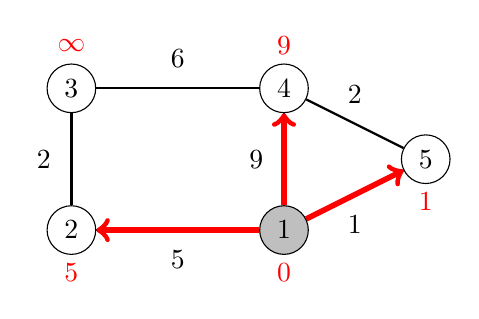
\begin{tikzpicture}[scale=0.9]
\node[draw, circle] (1) at (1,3) {3};
\node[draw, circle] (2) at (4,3) {4};
\node[draw, circle] (3) at (1,1) {2};
\node[draw, circle, fill=lightgray] (4) at (4,1) {1};
\node[draw, circle] (5) at (6,2) {5};

\node[color=red] at (1,3+0.6) {$\infty$};
\node[color=red] at (4,3+0.6) {$9$};
\node[color=red] at (1,1-0.6) {$5$};
\node[color=red] at (4,1-0.6) {$0$};
\node[color=red] at (6,2-0.6) {$1$};

\path[draw,thick,-] (1) -- node[font=\small,label=above:6] {} (2);
\path[draw,thick,-] (1) -- node[font=\small,label=left:2] {} (3);
\path[draw,thick,-] (3) -- node[font=\small,label=below:5] {} (4);
\path[draw,thick,-] (2) -- node[font=\small,label=left:9] {} (4);
\path[draw,thick,-] (2) -- node[font=\small,label=above:2] {} (5);
\path[draw,thick,-] (4) -- node[font=\small,label=below:1] {} (5);

\path[draw=red,thick,->,line width=2pt] (4) -- (2);
\path[draw=red,thick,->,line width=2pt] (4) -- (3);
\path[draw=red,thick,->,line width=2pt] (4) -- (5);
\end{tikzpicture}
\end{center}

この場合、ノード1からのエッジによって、ノード2、4、5の距離が更新され、その距離は5、9、1になりました。
次の処理ノードは、距離 1 のノード 5 です。
これを処理すると、ノード4までの距離が9から3になりました。

\begin{center}
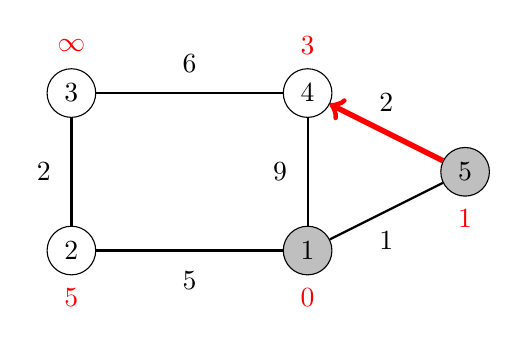
\begin{tikzpicture}
\node[draw, circle] (1) at (1,3) {3};
\node[draw, circle] (2) at (4,3) {4};
\node[draw, circle] (3) at (1,1) {2};
\node[draw, circle, fill=lightgray] (4) at (4,1) {1};
\node[draw, circle, fill=lightgray] (5) at (6,2) {5};

\node[color=red] at (1,3+0.6) {$\infty$};
\node[color=red] at (4,3+0.6) {$3$};
\node[color=red] at (1,1-0.6) {$5$};
\node[color=red] at (4,1-0.6) {$0$};
\node[color=red] at (6,2-0.6) {$1$};

\path[draw,thick,-] (1) -- node[font=\small,label=above:6] {} (2);
\path[draw,thick,-] (1) -- node[font=\small,label=left:2] {} (3);
\path[draw,thick,-] (3) -- node[font=\small,label=below:5] {} (4);
\path[draw,thick,-] (2) -- node[font=\small,label=left:9] {} (4);
\path[draw,thick,-] (2) -- node[font=\small,label=above:2] {} (5);
\path[draw,thick,-] (4) -- node[font=\small,label=below:1] {} (5);

\path[draw=red,thick,->,line width=2pt] (5) -- (2);
\end{tikzpicture}
\end{center}

次はノード4であり、ノード3までの距離が9になりました。

\begin{center}
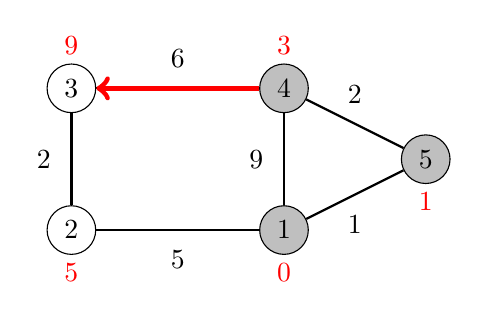
\begin{tikzpicture}[scale=0.9]
\node[draw, circle] (1) at (1,3) {3};
\node[draw, circle, fill=lightgray] (2) at (4,3) {4};
\node[draw, circle] (3) at (1,1) {2};
\node[draw, circle, fill=lightgray] (4) at (4,1) {1};
\node[draw, circle, fill=lightgray] (5) at (6,2) {5};

\node[color=red] at (1,3+0.6) {$9$};
\node[color=red] at (4,3+0.6) {$3$};
\node[color=red] at (1,1-0.6) {$5$};
\node[color=red] at (4,1-0.6) {$0$};
\node[color=red] at (6,2-0.6) {$1$};

\path[draw,thick,-] (1) -- node[font=\small,label=above:6] {} (2);
\path[draw,thick,-] (1) -- node[font=\small,label=left:2] {} (3);
\path[draw,thick,-] (3) -- node[font=\small,label=below:5] {} (4);
\path[draw,thick,-] (2) -- node[font=\small,label=left:9] {} (4);
\path[draw,thick,-] (2) -- node[font=\small,label=above:2] {} (5);
\path[draw,thick,-] (4) -- node[font=\small,label=below:1] {} (5);

\path[draw=red,thick,->,line width=2pt] (2) -- (1);
\end{tikzpicture}
\end{center}

ダイクストラ法で注目する特徴は、あるノードの処理を開始するときはいつでも、
その距離が最終的なものであることです。
例えば、この時点では、距離0、1、3がノード1、5、4への最終的な距離である。

このように、処理を続け、最終的な距離 は以下のようになります。

\begin{center}
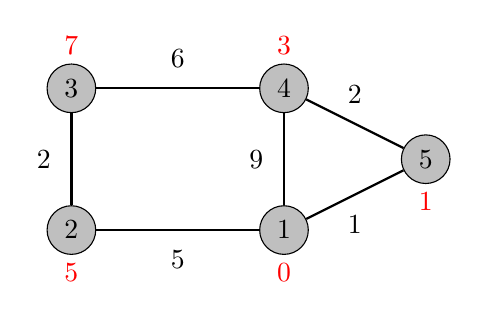
\begin{tikzpicture}[scale=0.9]
\node[draw, circle, fill=lightgray] (1) at (1,3) {3};
\node[draw, circle, fill=lightgray] (2) at (4,3) {4};
\node[draw, circle, fill=lightgray] (3) at (1,1) {2};
\node[draw, circle, fill=lightgray] (4) at (4,1) {1};
\node[draw, circle, fill=lightgray] (5) at (6,2) {5};

\node[color=red] at (1,3+0.6) {$7$};
\node[color=red] at (4,3+0.6) {$3$};
\node[color=red] at (1,1-0.6) {$5$};
\node[color=red] at (4,1-0.6) {$0$};
\node[color=red] at (6,2-0.6) {$1$};

\path[draw,thick,-] (1) -- node[font=\small,label=above:6] {} (2);
\path[draw,thick,-] (1) -- node[font=\small,label=left:2] {} (3);
\path[draw,thick,-] (3) -- node[font=\small,label=below:5] {} (4);
\path[draw,thick,-] (2) -- node[font=\small,label=left:9] {} (4);
\path[draw,thick,-] (2) -- node[font=\small,label=above:2] {} (5);
\path[draw,thick,-] (4) -- node[font=\small,label=below:1] {} (5);
\end{tikzpicture}
\end{center}

\subsubsection{Negative edges}

ダイクストラのアルゴリズムの効率性は、グラフに負のエッジが含まれないことを前提にしています。
もし、負の辺があると、アルゴリズムは正しくない結果を出す可能性があります。これを次のようなグラフで考えてみましょう。

\begin{center}
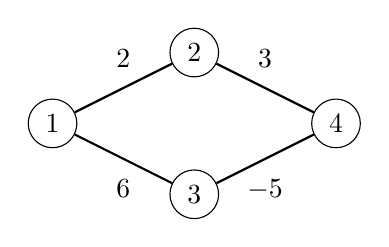
\begin{tikzpicture}[scale=0.9]
\node[draw, circle] (1) at (0,0) {$1$};
\node[draw, circle] (2) at (2,1) {$2$};
\node[draw, circle] (3) at (2,-1) {$3$};
\node[draw, circle] (4) at (4,0) {$4$};

\path[draw,thick,-] (1) -- node[font=\small,label=above:2] {} (2);
\path[draw,thick,-] (2) -- node[font=\small,label=above:3] {} (4);
\path[draw,thick,-] (1) -- node[font=\small,label=below:6] {} (3);
\path[draw,thick,-] (3) -- node[font=\small,label=below:$-5$] {} (4);
\end{tikzpicture}
\end{center}
\noindent
ノード1からノード4への最短経路は
$1 \rightarrow 3 \rightarrow 4$
で、その長さは1である。
しかし、ダイクストラのアルゴリズムでは最小の辺を辿って
$1 \rightarrow 2 \rightarrow 4$
の経路と確定します。
このケースでは、重み6のあとに重み-5があることが考慮されません。

\subsubsection{実装}

以下に実装を示します。
グラフは隣接リストとして保存され、ノード$a$からノード$b$に重み$w$のエッジがあるとき、 \texttt{adj[a]}には$(b, w)$のペアが含まれているとします。
ダイクストラ法を効率的に実装するには未処理の最小距離のノードを効率的に見つけることが可能であることが最も重要です。
このために距離でソートノードを含む優先度付きキュー(priority queue)を用います。
優先度付きキューを用いると、次に処理されるノードを対数時間(log)で検索することができます。
以下のコードでは,優先度付きキュー\texttt{q}は,
ノード$x$までの現在の距離が$d$であることを意味する,$(-d, x)$という形のpairを持ちます。
配列\texttt{distance}は
各ノードまでの距離を含み,
配列\texttt{processed}は
ノードが処理されたかどうかを持ちます。
初期状態では,$x$に対する距離は0であり,それ以外のノードに対する距離は$\infty$ です。
\begin{lstlisting}
for (int i = 1; i <= n; i++) distance[i] = INF;
distance[x] = 0;
q.push({0,x});
while (!q.empty()) {
    int a = q.top().second; q.pop();
    if (processed[a]) continue;
    processed[a] = true;
    for (auto u : adj[a]) {
        int b = u.first, w = u.second;
        if (distance[a]+w < distance[b]) {
            distance[b] = distance[a]+w;
            q.push({-distance[b],b});
        }
    }
}
\end{lstlisting}


優先度付きキューには,ノードへの距離をマイナスで保持しています。
C++のデフォルトの優先度付きキューは最大要素を返すので,最小要素を見つけるために負の距離を使用することで、デフォルトの優先度キューを直接使用することができます
\footnote{Of
course, we could also declare the priority queue as in Chapter 4.5
and use positive distances, but the implementation would be a bit longer.}。
また注意すべき点として、このキューには同じノードの処理待ちが入ることがありますが、距離が最小のもののみを処理すれば良いです。

このアルゴリズムは、すべてのノードを処理し、各エッジに対して最大で1つの情報を優先順位キューに追加するため、上記の実装の時間計算量は$O(n + m log m)$となります。

\section{ワーシャルフロイド法 - Floyd–Warshall algorithm}

\index{Floyd–Warshall algorithm}

このアルゴリズムでは、ノード間の距離を含む2次元の配列を保持する。まず、ノード間の直接のエッジのみを用いて距離を計算し、この後、アルゴリズムがパス中の中間ノードを用いて距離を縮める。
例

\key{ワーシャルフロイド法}\footnote{The algorithm
is named after R. W. Floyd and S. Warshall
who published it independently in 1962 \cite{flo62,war62}.}
は最短経路を求めるアルゴリズムですがこれまでの2つとはまた違ったアプローチです。
1回の実行でグラフ上の全ての2点の最短経路を求めることができます(訳註:これまではある始点からの距離を求めていたことに注意してください)。

ワーシャルフロイド法では、ノード間の距離を含む2次元の配列を保持します。
まず、ノード間の直接のエッジのみを用いて距離を更新し、経由するノードを用いて距離を更新するというアプローチを取ります。

\subsubsection{例}
以下のグラフでこの動きをみていきます。

\begin{center}
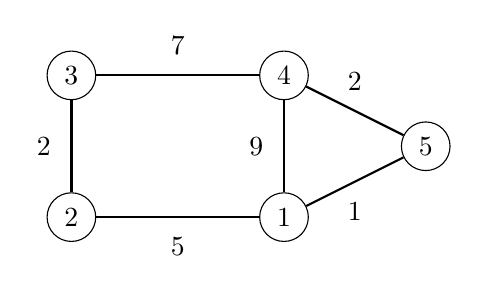
\begin{tikzpicture}[scale=0.9]
\node[draw, circle] (1) at (1,3) {$3$};
\node[draw, circle] (2) at (4,3) {$4$};
\node[draw, circle] (3) at (1,1) {$2$};
\node[draw, circle] (4) at (4,1) {$1$};
\node[draw, circle] (5) at (6,2) {$5$};

\path[draw,thick,-] (1) -- node[font=\small,label=above:7] {} (2);
\path[draw,thick,-] (1) -- node[font=\small,label=left:2] {} (3);
\path[draw,thick,-] (3) -- node[font=\small,label=below:5] {} (4);
\path[draw,thick,-] (2) -- node[font=\small,label=left:9] {} (4);
\path[draw,thick,-] (2) -- node[font=\small,label=above:2] {} (5);
\path[draw,thick,-] (4) -- node[font=\small,label=below:1] {} (5);
\end{tikzpicture}
\end{center}

初期状態では,各ノードからそれ自身への距離は$0$とします。ノード$a$とノード$b$の間に重み$x$をの辺が存在する場合,その距離は$x$です。
それ以外の配列の要素は$INF$とします。
このグラフにおいて、初期配列は次のようになります。

\begin{center}
\begin{tabular}{r|rrrrr}
 & 1 & 2 & 3 & 4 & 5 \\
\hline
1 & 0 & 5 & $\infty$ & 9 & 1 \\
2 & 5 & 0 & 2 & $\infty$ & $\infty$ \\
3 & $\infty$ & 2 & 0 & 7 & $\infty$ \\
4 & 9 & $\infty$ & 7 & 0 & 2 \\
5 & 1 & $\infty$ & $\infty$ & 2 & 0 \\
\end{tabular}
\end{center}
\vspace{10pt}

このアルゴリズムは同じ操作を複数のラウンド実行します。
各ラウンドにおいて、アルゴリズムは、パスの新しい中間ノードを選択し、このノードを用いて距離を減少させます。

第1ラウンドでは、ノード1が新しい中間ノードとします。
ノード 2 とノード 4 の間には、ノード 1 が接続しているため、長さ 14 の新しいパスがあります。
ノード2とノード5の間にも、長さ6の新しいパスがあります。

\begin{center}
\begin{tabular}{r|rrrrr}
 & 1 & 2 & 3 & 4 & 5 \\
\hline
1 & 0 & 5 & $\infty$ & 9 & 1 \\
2 & 5 & 0 & 2 & \textbf{14} & \textbf{6} \\
3 & $\infty$ & 2 & 0 & 7 & $\infty$ \\
4 & 9 & \textbf{14} & 7 & 0 & 2 \\
5 & 1 & \textbf{6} & $\infty$ & 2 & 0 \\
\end{tabular}
\end{center}
\vspace{10pt}


2ラウンド目では、ノード2が新たな中間ノードとします。
これにより、ノード1とノード3の間、ノード3とノード5の間に新しいパスができます。

\begin{center}
\begin{tabular}{r|rrrrr}
 & 1 & 2 & 3 & 4 & 5 \\
\hline
1 & 0 & 5 & \textbf{7} & 9 & 1 \\
2 & 5 & 0 & 2 & 14 & 6 \\
3 & \textbf{7} & 2 & 0 & 7 & \textbf{8} \\
4 & 9 & 14 & 7 & 0 & 2 \\
5 & 1 & 6 & \textbf{8} & 2 & 0 \\
\end{tabular}
\end{center}
\vspace{10pt}


3ラウンド目では、ノード3が新しい中間ラウンドとします。
ノード2と4の間に新しいパスができます。

\begin{center}
\begin{tabular}{r|rrrrr}
 & 1 & 2 & 3 & 4 & 5 \\
\hline
1 & 0 & 5 & 7 & 9 & 1 \\
2 & 5 & 0 & 2 & \textbf{9} & 6 \\
3 & 7 & 2 & 0 & 7 & 8 \\
4 & 9 & \textbf{9} & 7 & 0 & 2 \\
5 & 1 & 6 & 8 & 2 & 0 \\
\end{tabular}
\end{center}
\vspace{10pt}



このアルゴリズムは、すべてのノードが中間ノードに任命されるまで、このように続けられます(訳註: 上記の例のように$i$ラウンド目にはノード$i$が中間ノードとして計算します)。
アルゴリズムが終了すると,配列には任意の2つのノード間の最小距離が格納されています。

\begin{center}
\begin{tabular}{r|rrrrr}
 & 1 & 2 & 3 & 4 & 5 \\
\hline
1 & 0 & 5 & 7 & 3 & 1 \\
2 & 5 & 0 & 2 & 8 & 6 \\
3 & 7 & 2 & 0 & 7 & 8 \\
4 & 3 & 8 & 7 & 0 & 2 \\
5 & 1 & 6 & 8 & 2 & 0 \\
\end{tabular}
\end{center}



例えば,この結果から,ノード2とノード4の間の最短距離は8であることがわかります。これを次に示します。

\begin{center}
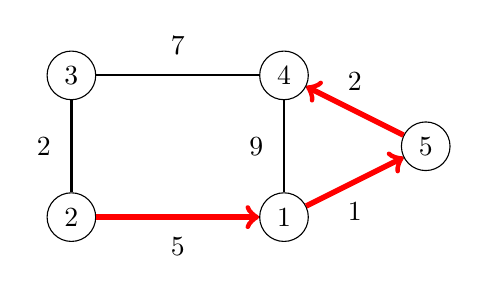
\begin{tikzpicture}[scale=0.9]
\node[draw, circle] (1) at (1,3) {$3$};
\node[draw, circle] (2) at (4,3) {$4$};
\node[draw, circle] (3) at (1,1) {$2$};
\node[draw, circle] (4) at (4,1) {$1$};
\node[draw, circle] (5) at (6,2) {$5$};

\path[draw,thick,-] (1) -- node[font=\small,label=above:7] {} (2);
\path[draw,thick,-] (1) -- node[font=\small,label=left:2] {} (3);
\path[draw,thick,-] (3) -- node[font=\small,label=below:5] {} (4);
\path[draw,thick,-] (2) -- node[font=\small,label=left:9] {} (4);
\path[draw,thick,-] (2) -- node[font=\small,label=above:2] {} (5);
\path[draw,thick,-] (4) -- node[font=\small,label=below:1] {} (5);

\path[draw=red,thick,->,line width=2pt] (3) -- (4);
\path[draw=red,thick,->,line width=2pt] (4) -- (5);
\path[draw=red,thick,->,line width=2pt] (5) -- (2);
\end{tikzpicture}
\end{center}

\subsubsection{実装}

このアルゴリズムの利点は、実装が簡単なことです。
以下のコードは、$\texttt{distance}[a][b]$をノード $a$ と $b$ 間の最短距離とする距離行列とします。
まず、この実装にはグラフの隣接行列  \texttt{adj} で辺の情報を与えます。

\begin{lstlisting}
for (int i = 1; i <= n; i++) {
    for (int j = 1; j <= n; j++) {
        if (i == j) distance[i][j] = 0;
        else if (adj[i][j]) distance[i][j] = adj[i][j];
        else distance[i][j] = INF;
    }
}
\end{lstlisting}
この後,以下のようにして最短距離を求めます。
\begin{lstlisting}
for (int k = 1; k <= n; k++) {
    for (int i = 1; i <= n; i++) {
        for (int j = 1; j <= n; j++) {
            distance[i][j] = min(distance[i][j],
                                   distance[i][k]+distance[k][j]);
        }
    }
}
\end{lstlisting}


このアルゴリズムは、グラフのノードを通過する3つの入れ子ループを含むため、時間計算量は$O(n^3)$です。

この実装は単純なので、グラフの最短経路を1つだけ見つける必要がある場合でも、このアルゴリズムは使用できます。
ただし、このアルゴリズムが使えるのは、グラフが非常に小さく、3乗の時間計算量で十分速くなる場合です。
